\documentclass[12pt]{article}

  % Get right packages
  \usepackage{amsmath}
  \usepackage{amssymb}
  \usepackage{amsthm}
  \usepackage{float}
  \usepackage{fullpage} % Package to use full page
  \usepackage{graphicx}
  \usepackage{hyperref}
  \usepackage{parskip} % Package to tweak paragraph skipping

  % User commands
  \newtheorem{thm}{Theorem}
  \DeclareMathOperator*{\argmax}{argmax}

  % Title info
  \title{Taxation Notes}
  \author{UMA Project}
  \date{\today}

\begin{document}

\maketitle

\clearpage
\newpage


\section{Non-technical Summary}

  The UMA Data Verification Machine (DVM) is responsible for producing ``honest'' prices that can be
  used to evaluate financial smart contracts on the blockchain. The DVM relies on votes by
  individuals who own UMA vote tokens to accurately report prices from the fiat world. In order to
  ensure that the DVM cannot be manipulated for financial gain, we must prove that it is
  economically not profitable to corrupt the system by purchasing enough tokens to corrupt the DVM
  by voting dishonestly.

  The tool we use to incentivize honest behavior is to tax the margin held in the financial smart
  contracts and use this margin to conduct buybacks of the UMA vote tokens. We view these buybacks
  as a way to ensure that there are returns paid to holding vote tokens and we prevent corruption
  by ensuring that the expected present discounted value of all future buybacks exceeds the amount
  that an individual could gain by corrupting the system. We build a mathematical model that
  describes these interactions and lay out the conditions necessary to ensure that there is no
  economically profitable corruption opportunities.

  We find that

  \begin{enumerate}
    \item Finding 1
    \item Finding 2
    \item Finding 3
  \end{enumerate}

  These findings motivate our proposed taxation structure

  \clearpage
  \newpage

\section{Technical Details}

  We now move on to describe the technical details of our findings.

  The core of argument will revolve around what we call the ``Profit from Corruption (PfC) less than
  Cost of Corruption (CoC)'' inequality ($PfC < CoC$). This inequality is meant to ensure that no
  one can profitably corrupt the DVM. We assume that the PfC is proportional to the amount of margin
  that is held in the system, $\text{PfC} = \gamma M_t$, and that the CoC is equal to buying
  sufficient vote tokens to corrupt the system\footnote{There are other types of attacks in which
  individuals can offer bribes to individual voters in order to incentivize them to corrupt the
  system --- We have other work in which we can show that the cheapest attack on our system involves
  a 51\% attack}, $\text{CoC} = \chi p_t S_t$ where $p_t$ denotes the dollar price of the UMA vote
  tokens and $S_t$ denotes the outstanding volume of tokens. We also rely on the assumption that
  market prices are accurate --- Namely that if $X_t$ are the dollar amounts of buybacks in each
  period $t$ and $r$ is the interest rate, then the market cap of the token would be
  $p_t S_t = E_t \left[ \sum_{s=0}^{\infty} \left(\frac{1}{1 + r}\right)^s X_t \right]$. Our
  standard assumption will be that the amount of margin that can be stolen is $\frac{1}{2}$ and the
  number of tokens required to corrupt is $\frac{1}{2}$.

  In each of the following subsections, we will use the notation presented below

  \begin{itemize}
    \item $B_t$ denotes the number of tokens bought back prior to vote
    \item $D_t$ denotes the dollar value of funds held in the ``rainy day fund''
    \item $M_t$ denotes total dollar value of margin in system
    \item $\tau_t$ denotes the tax rate on the system
    \item $p_t$ denotes the price of a single vote token
    \item $S_t$ denotes the number of vote tokens outstanding
    \item $T_t \equiv \tau_t M_t$ denotes total tax levied on system
    \item $X_t \equiv B_t p_t$ denotes the dollar value of expenditure on buybacks
  \end{itemize}

  Additionally the following are parameters

  \begin{itemize}
    \item $\chi$ is the fraction of voters required to corrupt the system
    \item $\eta$ is percent of people who do not vote
    \item $\gamma$ the fraction of margin seized if DVM is corrupted
    \item $\pi$ is the inflation rate used to reward voters
    \item $r$ is the risk-free return on other capital
  \end{itemize}

  The subsections that follow are

  \begin{itemize}
    \item Section \ref{sec:price_required} demonstrates the price that is required to prevent the
          system from being corrupted in any given period.
    \item Section \ref{sec:dss} asks the question, ``In a deterministic world in which the system
          margin has reached a steady level of margin, what is the lowest tax rate we can implement
          that ensure incorruptibility?'' We find that the lowest tax rate is the same as the return
          that we would like the tokens to offer.
    \item Section \ref{sec:dg} asks the question, ``If we knew exactly how margin would grow
          could charge in each period and maintain the incorruptibility gurantee starting today and
          going into the future, what is the minimum amount of taxes that we could impose at each
          period?'' We find that the rate of change in the tax rates is similar to the rate of
          change of the margin held in the system. We find that, under a particular
          parameterization, we can achieve a zero tax rate for almost 20 years before being required
          to increase taxes to steady state amounts.
    \item Section \ref{sec:sss} analyzes a model in which margin follows a stationary stochastic
          process and thinks about the right way to smooth taxes while making sure that payments
          can be made to ensure system is incorruptible.''
  \end{itemize}

  \subsection{Price required for $PfC < CoC$} \label{sec:price_required}
    %!TEX root = ../TaxationPlan.tex

In this section we express the price needed to maintain the $PfC < CoC$ inequality in terms of
model primitives:

We rearrange the inequality in the following manner

\begin{align*}
  PfC_t \leq CoC_t \\
  \Rightarrow \gamma M_t \leq \frac{1 - \eta}{2} p_t S_t \\
  \Rightarrow p_t \geq \frac{2}{1 - \eta} \frac{\gamma M_t}{S_t}
  \Rightarrow p_t \geq \frac{2}{1 - \eta} \frac{\gamma M_t}{S_t}
\end{align*}

Thus as long as the price of a token is higher than $\frac{2}{1 - \eta} \frac{\gamma M_t}{S_t}$,
then it is not profitable to corrupt the system.


  \subsection{Deterministic Steady State} \label{sec:dss}
    %!TEX root = ../TaxationPlan.tex

In this version of the model, we will consider the system margin being constant over time, i.e.
$M_t = \bar{M}$ $\forall t$. However, it is important to note that not all of the variables will be
constant in the steady state because there is potentially non-zero inflation in the number of
outstanding tokens.

The total number of tokens follows

\begin{align*}
  S_{t+1} &= (1 + \pi) (S_t - B_t)
\end{align*}

Also, recall that the price that ensures $PfC < CoC$ is given by
$p_t \geq \frac{2}{1 - \eta} \frac{PfC_t}{S_t}$.

The token market cap, $p_t S_t$, will be a constant since

\begin{align*}
  p_t S_t &= \frac{2}{1 - \eta} \frac{PfC_t}{S_t} S_t \\
  &= \frac{2}{1 - \eta} PfC_t \\
  &= \frac{2}{1 - \eta} \gamma M_t \\
  &= \frac{2}{1 - \eta} \gamma \bar{M}
\end{align*}

Assume that we'd like to achieve an aggregate period-by-period return of $r$ to token holders.

\begin{align*}
  (1 + r) &= \frac{p_{t+1} (S_{t+1} + B_{t+1})}{p_t S_t} \\
  (1 + r) &= \frac{p_{t+1} S_{t+1} + X_{t+1}}{p_t S_t} \\
  (1 + r) &= \frac{\frac{2}{1 - \eta} \frac{PfC_{t+1}}{S_{t+1}} S_{t+1} + X_{t+1}}{\frac{2}{1 - \eta} \frac{PfC_{t}}{S_t} S_t} \\
  (1 + r) PfC_{t} &= PfC_{t+1} + \frac{1 - \eta}{2} X_{t+1}
\end{align*}

In the SS this means that

\begin{align*}
  (1 + r) \bar{PfC} &= \bar{PfC} + \frac{1 - \eta}{2} \bar{X} \\
  &\rightarrow \bar{X} = \frac{2 \bar{PfC}}{1 - \eta} r
\end{align*}

If we assume that $\bar{PfC} = \frac{1}{2} \bar{M}$ and that there is full participation then this
reduces to $\bar{X} = r \bar{M}$ which means that the fee rate is given by,

$$\bar{\tau} \equiv \frac{\bar{X}}{\bar{M}} = r$$

The question of how high fees should be in the steady state depend on what one believes about the
return that token holders are willing to accept on their tokens.

If the following three things were true,

\begin{enumerate}
  \item Blockchains become a widely accepted and used technology
  \item UMA was core to decentralized finance
  \item People were confident that UMA would continue to be a core component of decentralized finance
\end{enumerate}

then it is feasible that token holders would accept interest rates near the risk-free rate. Under
current market conditions, this could translate into a required annualized fee rate of between 2\%
and 5\%, but, even in more ``investor friendly times,'' this should not exceed 5\%-10\%.


  \subsection{Determisitic Growth} \label{sec:dg}
    %!TEX root = ../TaxationPlan.tex

We now consider how to implement taxes in a world where the system margin grows over time
according to a deterministic process. One of the reasons that it is important to model growth in
this system is that, if people believe that there will be higher buybacks in the future, then we
might be able to sustain lower buybacks today.

For simplicity, we assume that margin follows

$$M_{t+1} = M_{t} + g M_{t} \left(1 + \frac{M_{t}}{\bar{M}} \right)$$

This process, known as logistic growth, generates ``S-shaped'' growth. We can see the implications
that this process has for the total system margin in Figure \ref{fig:dg_margin_growth}.

\begin{center}
  \begin{figure}[H]
    \scalebox{0.65}{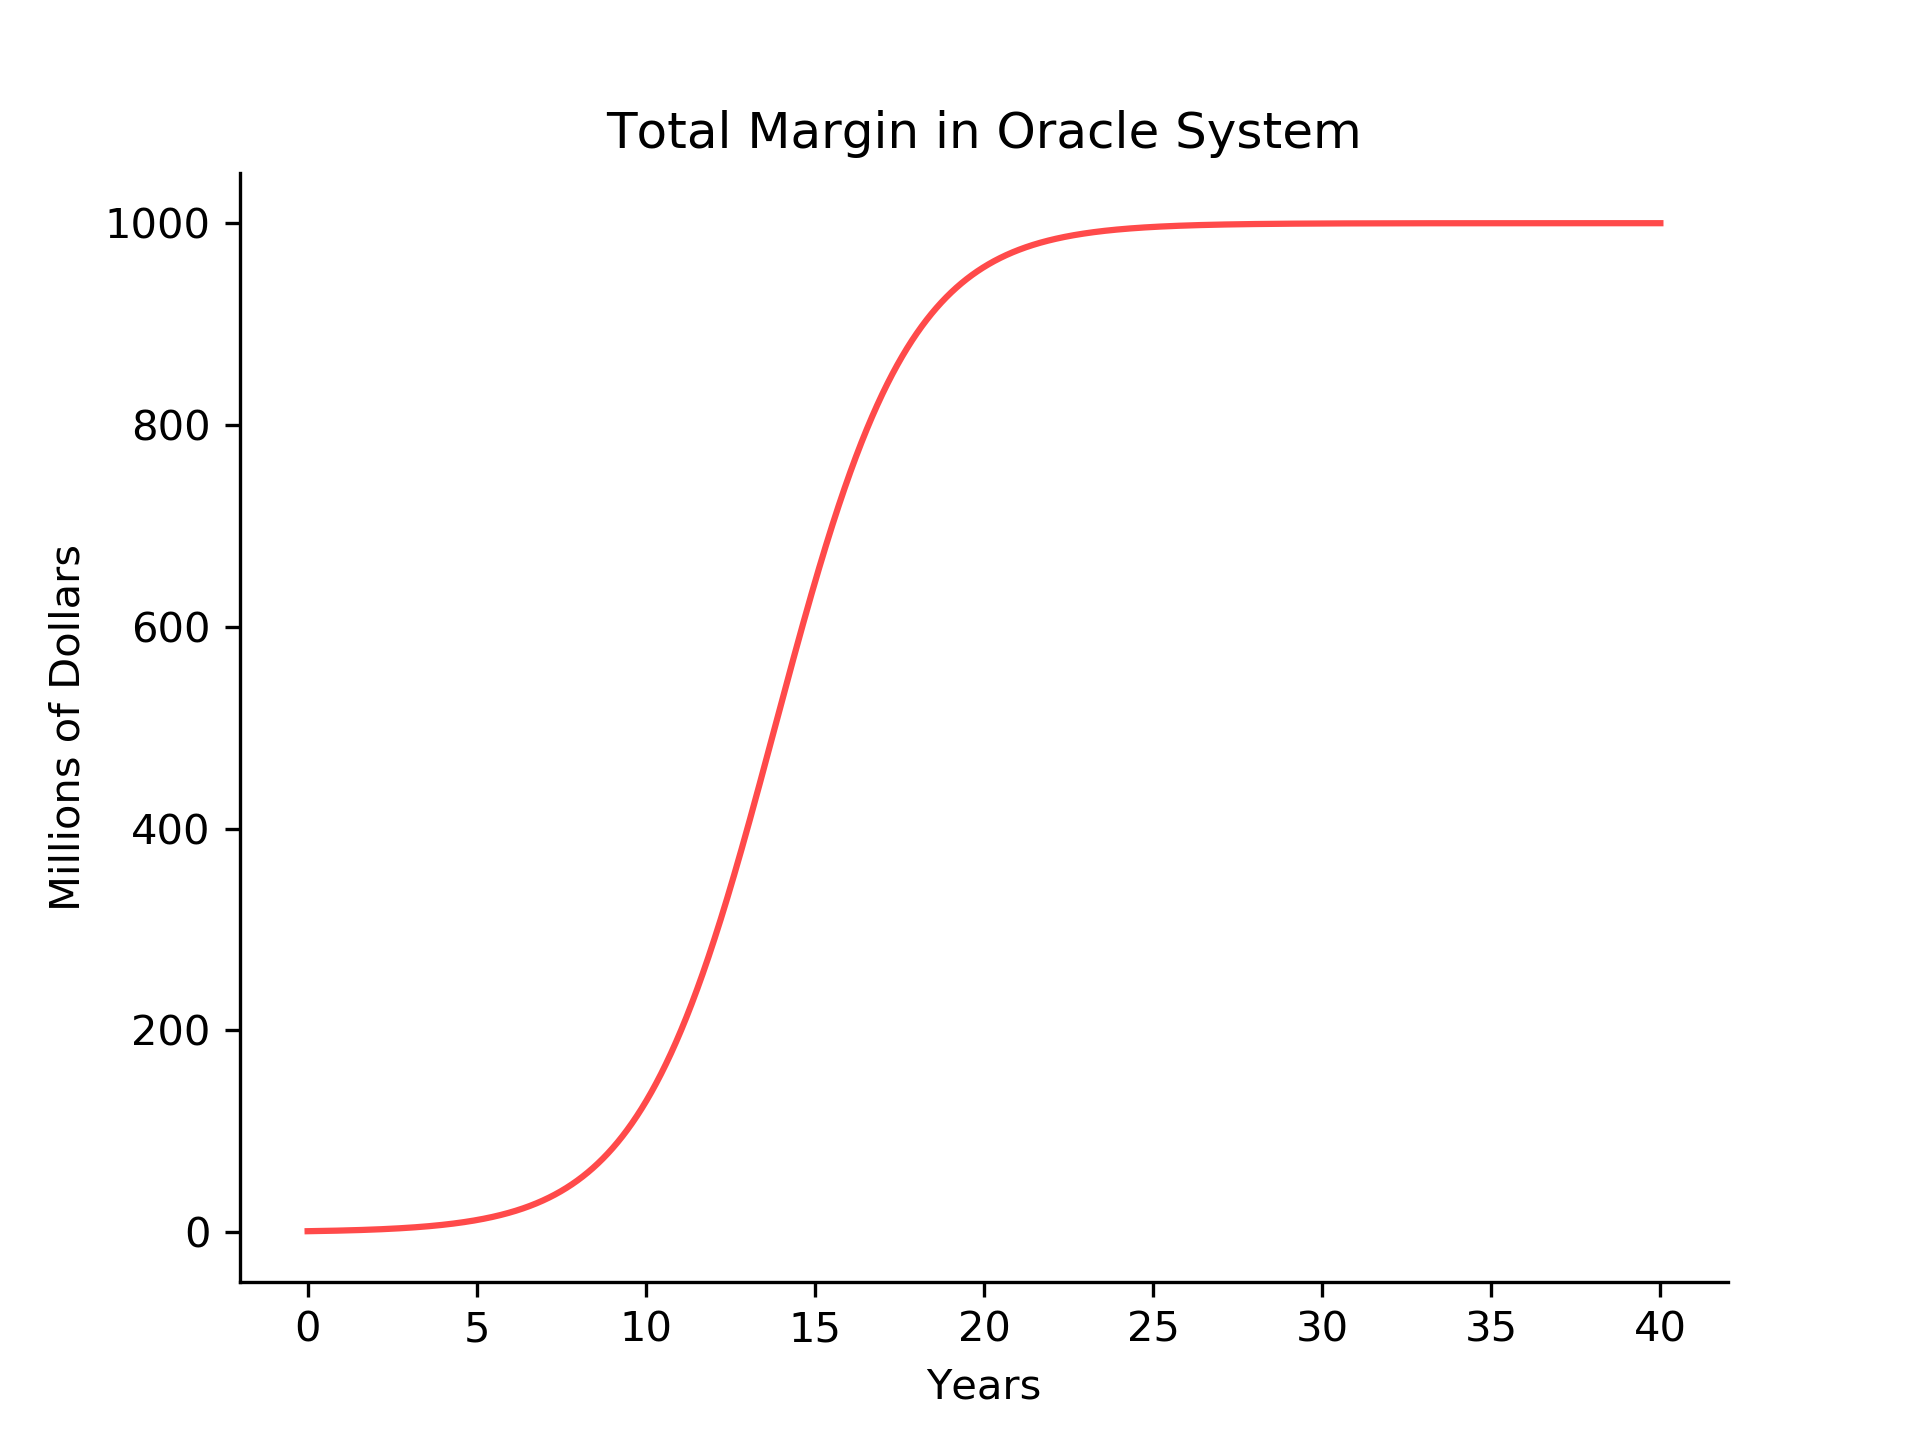
\includegraphics{./TaxationPlanImages/MarginGrowth.png}}
    \label{fig:dg_margin_growth}
  \end{figure}
\end{center}

We assume that we would like to charge the minimum amount of taxes while maintaining the system's
incorruptibility. This produces the following mathematical program:

\begin{align*}
  \min_{T_t} \; &E \left[ \sum_{t=0} \left(\frac{1}{1 + r} \right)^t T_t \right] \\
  &\text{subject to} \\
  PfC_t &\leq \frac{1}{2} P_t S_t = \frac{1}{2} E \left[ \sum_{s=0} \left(\frac{1}{1 + r}\right)^s  X_{t + s} \right] \\
  X_{t} &= T_t \\
  0 &\leq T_t \\
  T_t &\leq \bar{\tau} \bar{M} \\
  M_{t+1} &= M_{t} + g M_{t} \left(1 + \frac{M_t}{\bar{M}} \right)
\end{align*}

We can solve this program indirectly by choosing an $s$ such that $M_s \approx \bar{M}$. At this
point, we have arrived in the steady state and the tax rate implemented will be
$T_t = \bar{\tau} M_t$. We can then step back by one period to $t = s - 1$ and compute what the
required $X_t$ in that period would be. We can proceed to step this back until we reach our initial
condition of $M_0$ which traces out a path of tax collections. This process generates a sequence of
taxes that look like Figure \ref{fig:dg_tax_growth}.

\begin{center}
  \begin{figure}[H]
    \scalebox{0.65}{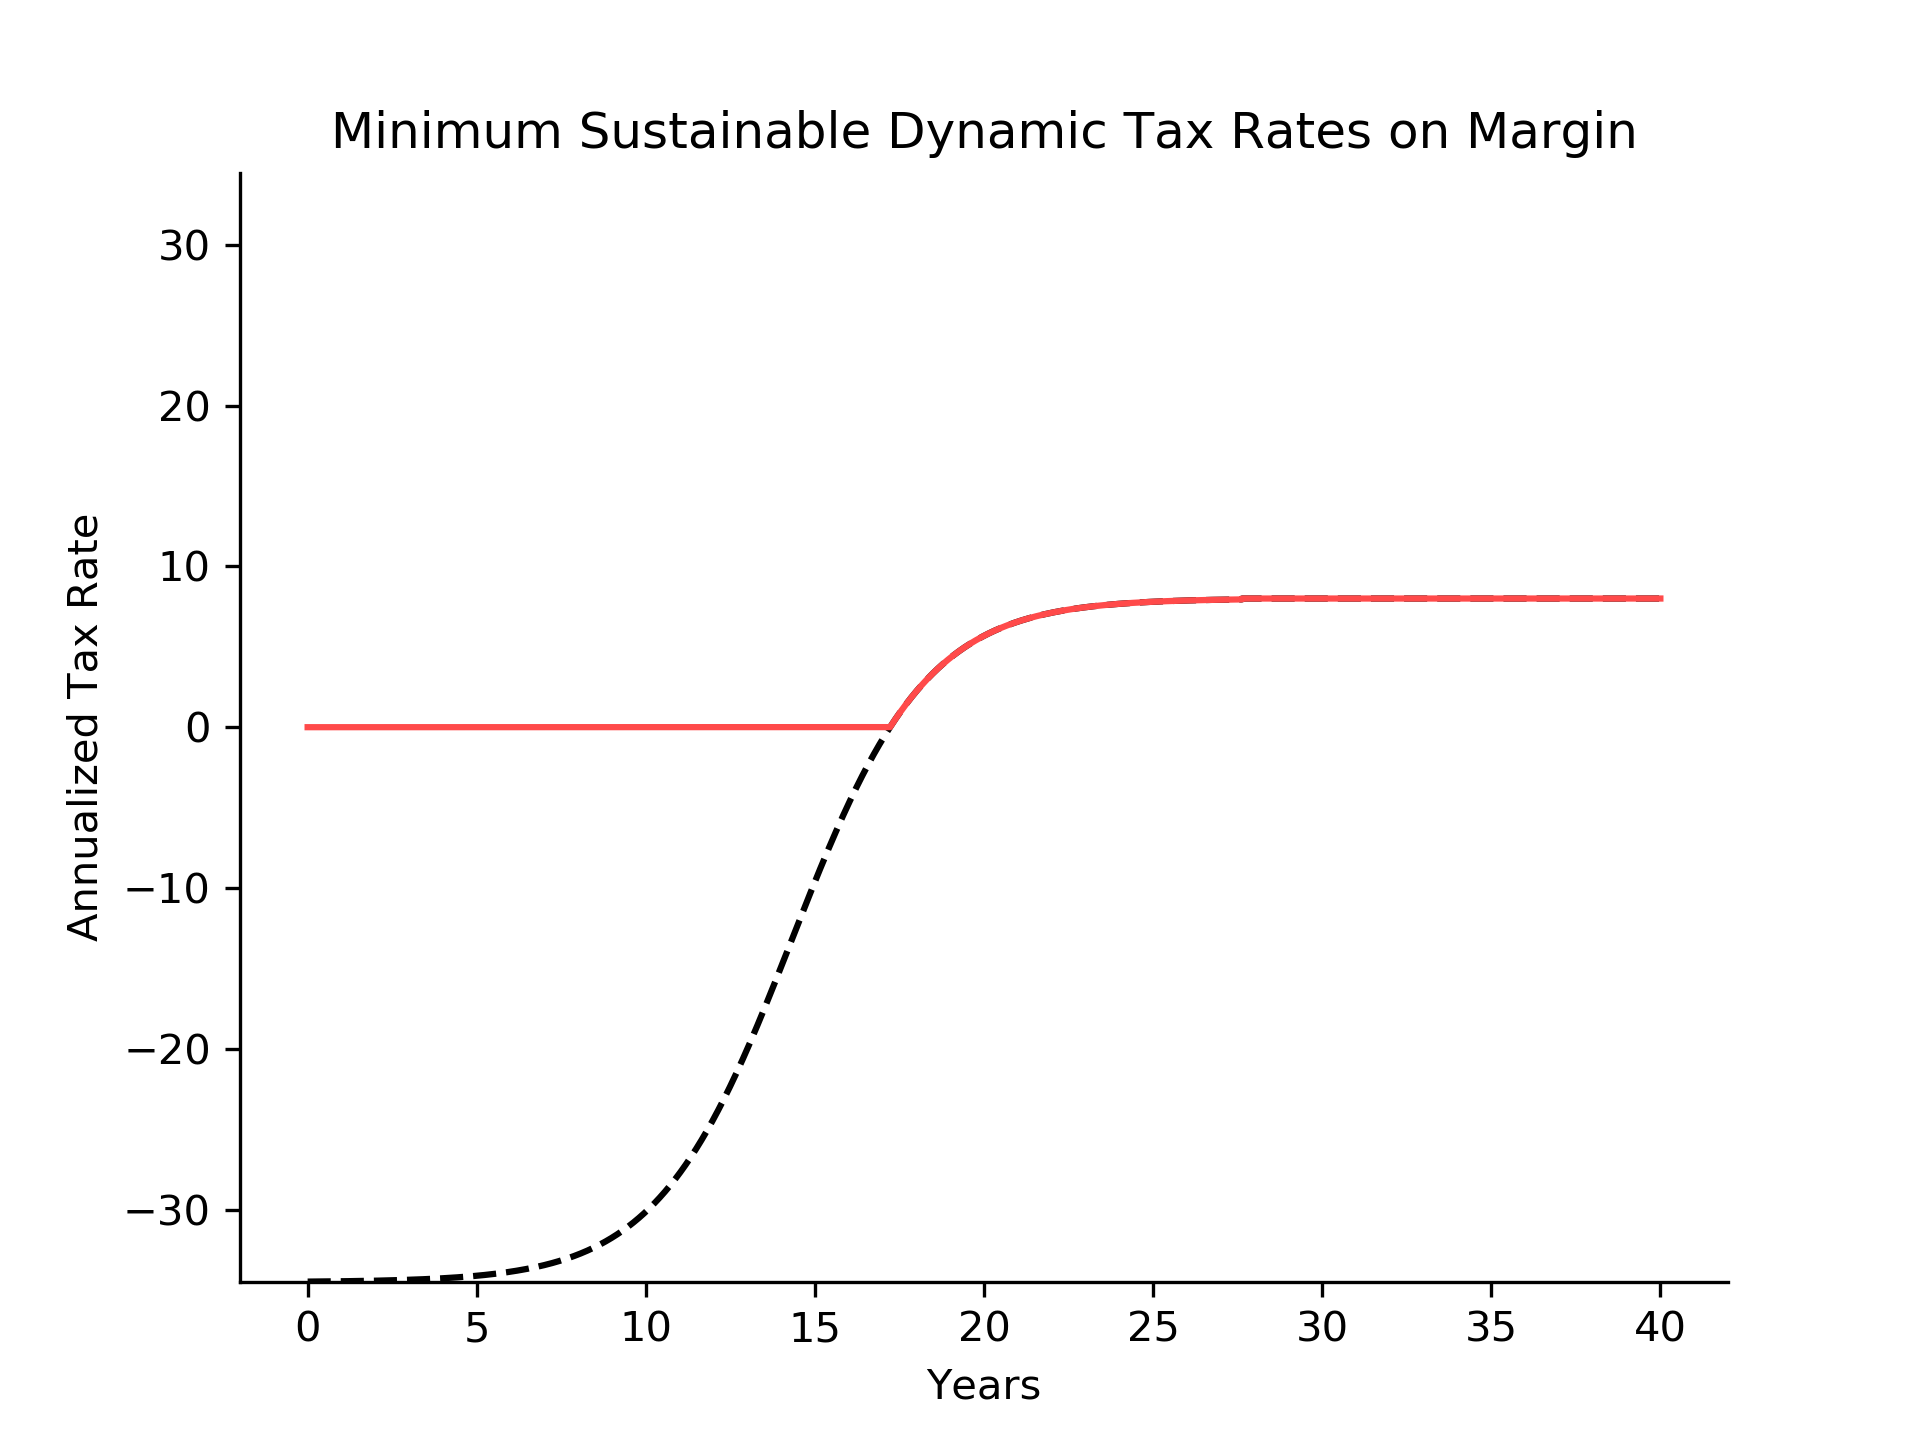
\includegraphics{./TaxationPlanImages/TaxRates.png}}
    \label{fig:dg_tax_growth}
  \end{figure}
\end{center}

We plot the solution to two different mathematical programs. The first, plotted as a solid line,
corresponds to the program that we described above. The second, plotted as a dashed line,
corresponds to what tax rates would be if we did not impose the non-negativity constraint. Notice
that in the case in which there is no non-negativity constraint, the taxes go negative in order to
meet the $PfC < CoC$ constraint with equality.

The most interesting observation we make from this chart is that taxes can start low and stay low
for a prolonged period of time before rising to the steady state levels. The reason that this
satisfies the $PfC < CoC$ inequality is that individuals understand that there will be growth in
the system --- The future promise of increased buybacks in the future is enough to secure the system
while it is new (and small).

We can be see this by looking at the equation that determines the $CoC$:

\begin{align*}
  CoC_t &= \chi p_t S_t = \chi E \left[ \sum_{s=0}^{\infty} \left(\frac{1}{1 + r} \right)^s X_{t+s} \right]
\end{align*}

High values of $X_{t + s}$ increase the cost of corruption in period $t$. This insight is somewhat
general, but may be potentially too strong in this model due to the fact that there is certainty
about the future growth. This concern motivates our next section in which we introduce uncertainty
about the growth of the system.


  \subsection{Stochastic Steady State} \label{sec:sss}
    %!TEX root = ../TaxationPlan.tex

In the deterministic model, there were no unexpected fluctuations or growth, and thus there was no
risk. Additionally, since margin was either constant or always growing, there was no reason to save
any of the margin collected to pay future taxes thus the amount taxed and the amount used for
buybacks were the same. In the stochastic analysis, this will cease to be true. We will now have to
consider how to structure the buybacks, $X_t$, and taxes, $T_t$, separately.

We will assume that margin follows a Markov process,

$$M_{t+1} = f(M_t, \varepsilon_{t+1})$$

Our objective will be to choose $\{(X_t, T_t)\}_{t=0}^{\infty}$ to optimize certain goals. In this
document, we will focus on minimizing the present discounted value of payouts to token holders and
minimizing the variance in the tax rates.

\textbf{Two Part Solution}

One way that we might consider solving this problem, that should provide a nearly optimal solution
is to break it into two parts:

\begin{enumerate}
  \item Solve for the minimum cost policy function $X^*(M^t)$
  \item Find the minimum variance tax function $T^*(M^t)$ such that we can fund any sequence of
        buybacks, $\{X(M^t)\}$, without debt
\end{enumerate}

Formally, the first step is the solution to

\begin{align*}
  \min_{\{X_t\}} \; & E \left[ \sum_{t} \left(\frac{1}{1 + r} \right) X_t \right] \\
  &\text{subject to} \\
  \quad & 2 PfC_t \leq E \left[ \sum_{s=0}^{\infty} \left(\frac{1}{1 + r}\right)^s X_{t+s} \right] \quad (\lambda_t)
\end{align*}

If we add the restriction that the policy is Markov, $X^*(M^t) = X^*(M_t)$, then we know

\begin{align*}
  2 \gamma M_t &\leq E \left[ \sum_{s=0}^{\infty} \left( \frac{1}{1+r} \right)^s X^*(M^s) \right] \\
  &\leq \sum_{s=0}^{\infty} \left( \frac{1}{1+r} \right)^s E \left[X^*(M_s) | M_t \right]
\end{align*}

It is easy to show that under the optimal solution that this inequality will hold with equality. If
we also assume that the process is a discrete Markov chain with transition matrix, $P$, then this
reduces to

\begin{align*}
  2 \gamma M_t &= \sum_{s=0}^{\infty} \left( \frac{1}{1+r} \right)^s E \left[X^*(M_s) | M_t \right] \\
  2 \gamma \vec{M} &= \sum_{s=0}^{\infty} \left( \frac{1}{1+r} \right)^s P^s \vec{X} \\
  &\dots \\
  \vec{X} &= 2 \gamma \left(I - \frac{1}{1 + r} P \right) \vec{M}
\end{align*}

We can then formalize the second step with

\begin{align*}
  \min_{\{T_t\}} \; & E \left[ \sum_{t} \left( \frac{1}{1 + r} \right)^t T_t^2 \right] \\
  &\text{subject to} \\
  T_t + (1 + r) D_t &\geq D_{t+1} + X^*_t \quad (\mu_t) \\
  D_t &\geq 0
\end{align*}

We can write this recursively as

\begin{align*}
  V(D_t, M_t) &= \max_{T_t} \; T_t^2 + \frac{1}{1 + r} E [V(D_{t+1}, M_{t+1})] \\
  &\text{Subject to} \\
  &D_{t+1} + X_{t} \leq (1 + r) D_t + T_t
\end{align*}

\subsubsection{Numerical Example}


  \subsection{Stochastic Growth} \label{sec:sg}


\end{document}
